% Options for packages loaded elsewhere
\PassOptionsToPackage{unicode}{hyperref}
\PassOptionsToPackage{hyphens}{url}
\PassOptionsToPackage{dvipsnames,svgnames,x11names}{xcolor}
%
\documentclass[
  letterpaper,
  DIV=11,
  numbers=noendperiod,
  oneside]{scrartcl}

\usepackage{amsmath,amssymb}
\usepackage{iftex}
\ifPDFTeX
  \usepackage[T1]{fontenc}
  \usepackage[utf8]{inputenc}
  \usepackage{textcomp} % provide euro and other symbols
\else % if luatex or xetex
  \usepackage{unicode-math}
  \defaultfontfeatures{Scale=MatchLowercase}
  \defaultfontfeatures[\rmfamily]{Ligatures=TeX,Scale=1}
\fi
\usepackage{lmodern}
\ifPDFTeX\else  
    % xetex/luatex font selection
\fi
% Use upquote if available, for straight quotes in verbatim environments
\IfFileExists{upquote.sty}{\usepackage{upquote}}{}
\IfFileExists{microtype.sty}{% use microtype if available
  \usepackage[]{microtype}
  \UseMicrotypeSet[protrusion]{basicmath} % disable protrusion for tt fonts
}{}
\makeatletter
\@ifundefined{KOMAClassName}{% if non-KOMA class
  \IfFileExists{parskip.sty}{%
    \usepackage{parskip}
  }{% else
    \setlength{\parindent}{0pt}
    \setlength{\parskip}{6pt plus 2pt minus 1pt}}
}{% if KOMA class
  \KOMAoptions{parskip=half}}
\makeatother
\usepackage{xcolor}
\usepackage[left=1in,marginparwidth=2.0666666666667in,textwidth=4.1333333333333in,marginparsep=0.3in]{geometry}
\setlength{\emergencystretch}{3em} % prevent overfull lines
\setcounter{secnumdepth}{-\maxdimen} % remove section numbering
% Make \paragraph and \subparagraph free-standing
\makeatletter
\ifx\paragraph\undefined\else
  \let\oldparagraph\paragraph
  \renewcommand{\paragraph}{
    \@ifstar
      \xxxParagraphStar
      \xxxParagraphNoStar
  }
  \newcommand{\xxxParagraphStar}[1]{\oldparagraph*{#1}\mbox{}}
  \newcommand{\xxxParagraphNoStar}[1]{\oldparagraph{#1}\mbox{}}
\fi
\ifx\subparagraph\undefined\else
  \let\oldsubparagraph\subparagraph
  \renewcommand{\subparagraph}{
    \@ifstar
      \xxxSubParagraphStar
      \xxxSubParagraphNoStar
  }
  \newcommand{\xxxSubParagraphStar}[1]{\oldsubparagraph*{#1}\mbox{}}
  \newcommand{\xxxSubParagraphNoStar}[1]{\oldsubparagraph{#1}\mbox{}}
\fi
\makeatother


\providecommand{\tightlist}{%
  \setlength{\itemsep}{0pt}\setlength{\parskip}{0pt}}\usepackage{longtable,booktabs,array}
\usepackage{calc} % for calculating minipage widths
% Correct order of tables after \paragraph or \subparagraph
\usepackage{etoolbox}
\makeatletter
\patchcmd\longtable{\par}{\if@noskipsec\mbox{}\fi\par}{}{}
\makeatother
% Allow footnotes in longtable head/foot
\IfFileExists{footnotehyper.sty}{\usepackage{footnotehyper}}{\usepackage{footnote}}
\makesavenoteenv{longtable}
\usepackage{graphicx}
\makeatletter
\def\maxwidth{\ifdim\Gin@nat@width>\linewidth\linewidth\else\Gin@nat@width\fi}
\def\maxheight{\ifdim\Gin@nat@height>\textheight\textheight\else\Gin@nat@height\fi}
\makeatother
% Scale images if necessary, so that they will not overflow the page
% margins by default, and it is still possible to overwrite the defaults
% using explicit options in \includegraphics[width, height, ...]{}
\setkeys{Gin}{width=\maxwidth,height=\maxheight,keepaspectratio}
% Set default figure placement to htbp
\makeatletter
\def\fps@figure{htbp}
\makeatother

% load packages
\usepackage{geometry}
\usepackage{xcolor}
\usepackage{eso-pic}
\usepackage{fancyhdr}
\usepackage{sectsty}
\usepackage{fontspec}
\usepackage{titlesec}

%% Set page size with a wider right margin
\geometry{a4paper, total={170mm,257mm}, left=20mm, top=20mm, bottom=20mm, right=50mm}

%% Let's define some colours
\definecolor{light}{HTML}{E6E6FA}
\definecolor{highlight}{HTML}{800080}
\definecolor{dark}{HTML}{330033}

%% Let's add the border on the right hand side 
\AddToShipoutPicture{% 
    \AtPageLowerLeft{% 
        \put(\LenToUnit{\dimexpr\paperwidth-3cm},0){% 
            \color{light}\rule{3cm}{\LenToUnit\paperheight}%
          }%
     }%
     % logo
    \AtPageLowerLeft{% start the bar at the bottom right of the page
        \put(\LenToUnit{\dimexpr\paperwidth-2.25cm},27.2cm){% move it to the top right
            \color{light}
\includegraphics[width=1.5cm]{_extensions/nrennie/PrettyPDF/logo.png}
          }%
     }%
}

%% Style the page number
\fancypagestyle{mystyle}{
  \fancyhf{}
  \renewcommand\headrulewidth{0pt}
  \fancyfoot[R]{\thepage}
  \fancyfootoffset{3.5cm}
}
\setlength{\footskip}{20pt}

%% style the chapter/section fonts
\chapterfont{\color{dark}\fontsize{20}{16.8}\selectfont}
\sectionfont{\color{dark}\fontsize{20}{16.8}\selectfont}
\subsectionfont{\color{dark}\fontsize{14}{16.8}\selectfont}
\titleformat{\subsection}
  {\sffamily\Large\bfseries}{\thesection}{1em}{}[{\titlerule[0.8pt]}]
  
% left align title
\makeatletter
\renewcommand{\maketitle}{\bgroup\setlength{\parindent}{0pt}
\begin{flushleft}
  {\sffamily\huge\textbf{\MakeUppercase{\@title}}} \vspace{0.3cm} \newline
  {\Large {\@subtitle}} \newline
  \@author
\end{flushleft}\egroup
}
\makeatother

%% Use some custom fonts
\setsansfont{Ubuntu}[
    Path=_extensions/nrennie/PrettyPDF/Ubuntu/,
    Scale=0.9,
    Extension = .ttf,
    UprightFont=*-Regular,
    BoldFont=*-Bold,
    ItalicFont=*-Italic,
    ]

\setmainfont{Ubuntu}[
    Path=_extensions/nrennie/PrettyPDF/Ubuntu/,
    Scale=0.9,
    Extension = .ttf,
    UprightFont=*-Regular,
    BoldFont=*-Bold,
    ItalicFont=*-Italic,
    ]
\KOMAoption{captions}{tableheading}
\makeatletter
\@ifpackageloaded{caption}{}{\usepackage{caption}}
\AtBeginDocument{%
\ifdefined\contentsname
  \renewcommand*\contentsname{Table of contents}
\else
  \newcommand\contentsname{Table of contents}
\fi
\ifdefined\listfigurename
  \renewcommand*\listfigurename{List of Figures}
\else
  \newcommand\listfigurename{List of Figures}
\fi
\ifdefined\listtablename
  \renewcommand*\listtablename{List of Tables}
\else
  \newcommand\listtablename{List of Tables}
\fi
\ifdefined\figurename
  \renewcommand*\figurename{Figure}
\else
  \newcommand\figurename{Figure}
\fi
\ifdefined\tablename
  \renewcommand*\tablename{Table}
\else
  \newcommand\tablename{Table}
\fi
}
\@ifpackageloaded{float}{}{\usepackage{float}}
\floatstyle{ruled}
\@ifundefined{c@chapter}{\newfloat{codelisting}{h}{lop}}{\newfloat{codelisting}{h}{lop}[chapter]}
\floatname{codelisting}{Listing}
\newcommand*\listoflistings{\listof{codelisting}{List of Listings}}
\makeatother
\makeatletter
\makeatother
\makeatletter
\@ifpackageloaded{caption}{}{\usepackage{caption}}
\@ifpackageloaded{subcaption}{}{\usepackage{subcaption}}
\makeatother
\makeatletter
\@ifpackageloaded{tcolorbox}{}{\usepackage[skins,breakable]{tcolorbox}}
\makeatother
\makeatletter
\@ifundefined{shadecolor}{\definecolor{shadecolor}{rgb}{.97, .97, .97}}{}
\makeatother
\makeatletter
\@ifundefined{codebgcolor}{\definecolor{codebgcolor}{named}{light}}{}
\makeatother
\makeatletter
\ifdefined\Shaded\renewenvironment{Shaded}{\begin{tcolorbox}[sharp corners, enhanced, boxrule=0pt, colback={codebgcolor}, breakable, frame hidden]}{\end{tcolorbox}}\fi
\makeatother
\makeatletter
\@ifpackageloaded{sidenotes}{}{\usepackage{sidenotes}}
\@ifpackageloaded{marginnote}{}{\usepackage{marginnote}}
\makeatother

\ifLuaTeX
  \usepackage{selnolig}  % disable illegal ligatures
\fi
\usepackage{bookmark}

\IfFileExists{xurl.sty}{\usepackage{xurl}}{} % add URL line breaks if available
\urlstyle{same} % disable monospaced font for URLs
\hypersetup{
  colorlinks=true,
  linkcolor={highlight},
  filecolor={Maroon},
  citecolor={Blue},
  urlcolor={highlight},
  pdfcreator={LaTeX via pandoc}}


\author{}
\date{}

\begin{document}

\pagestyle{mystyle}


\subsection{W1: Content}\label{w1-content}

\href{https://emerson.edu/faculty-staff-directory/kate-eichhorn}{Kate
Eichhorn}, \textbf{Content}:

\begin{itemize}
\tightlist
\item
  ``\href{pdf/eichhorn-content-ch1.pdf}{A Brief History of Content in a
  Digital Era}''
\item
  ``\href{pdf/eichhorn-content-ch2.pdf}{User-Generated Content}''
  (recommended)
\end{itemize}

\marginnote{\begin{footnotesize}

\href{https://www.instagram.com/world_record_egg/}{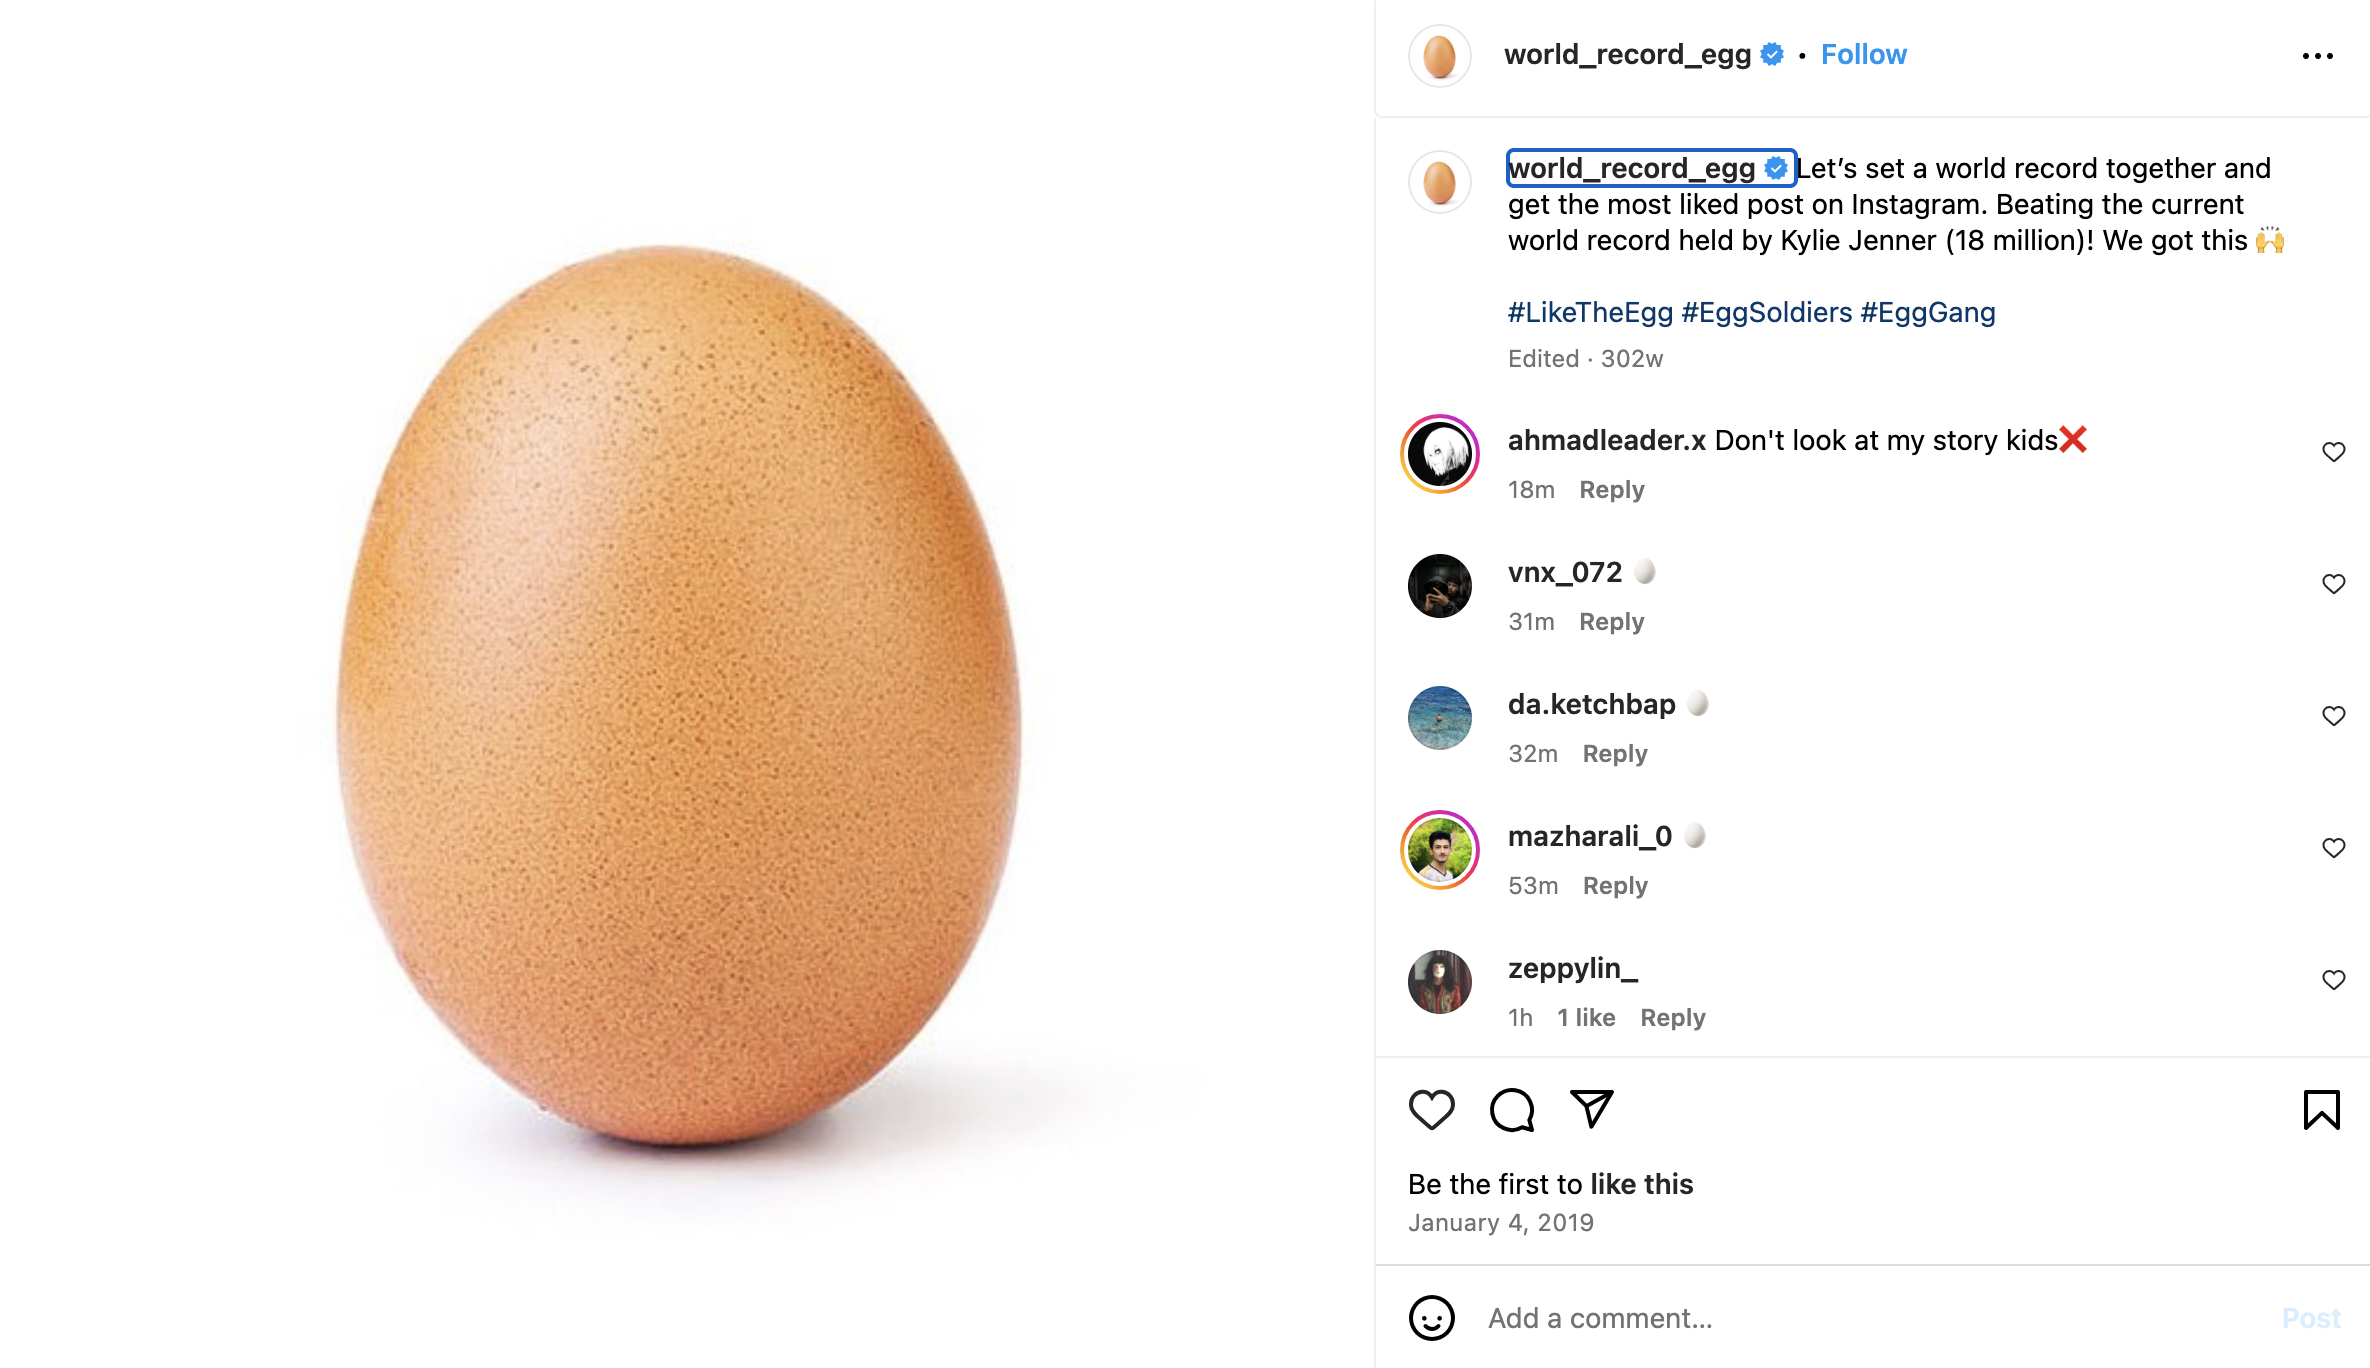
\includegraphics{img/egg.jpeg}}

\end{footnotesize}}

See also: Patrick H. Willems,
``\href{https://youtu.be/hAtbFwzZp6Y}{Everything is Content Now}''
(YouTube)

\begin{center}\rule{0.5\linewidth}{0.5pt}\end{center}

\subsection{Infinite Content}\label{infinite-content}

\href{https://www.netflix.com/title/70153373}{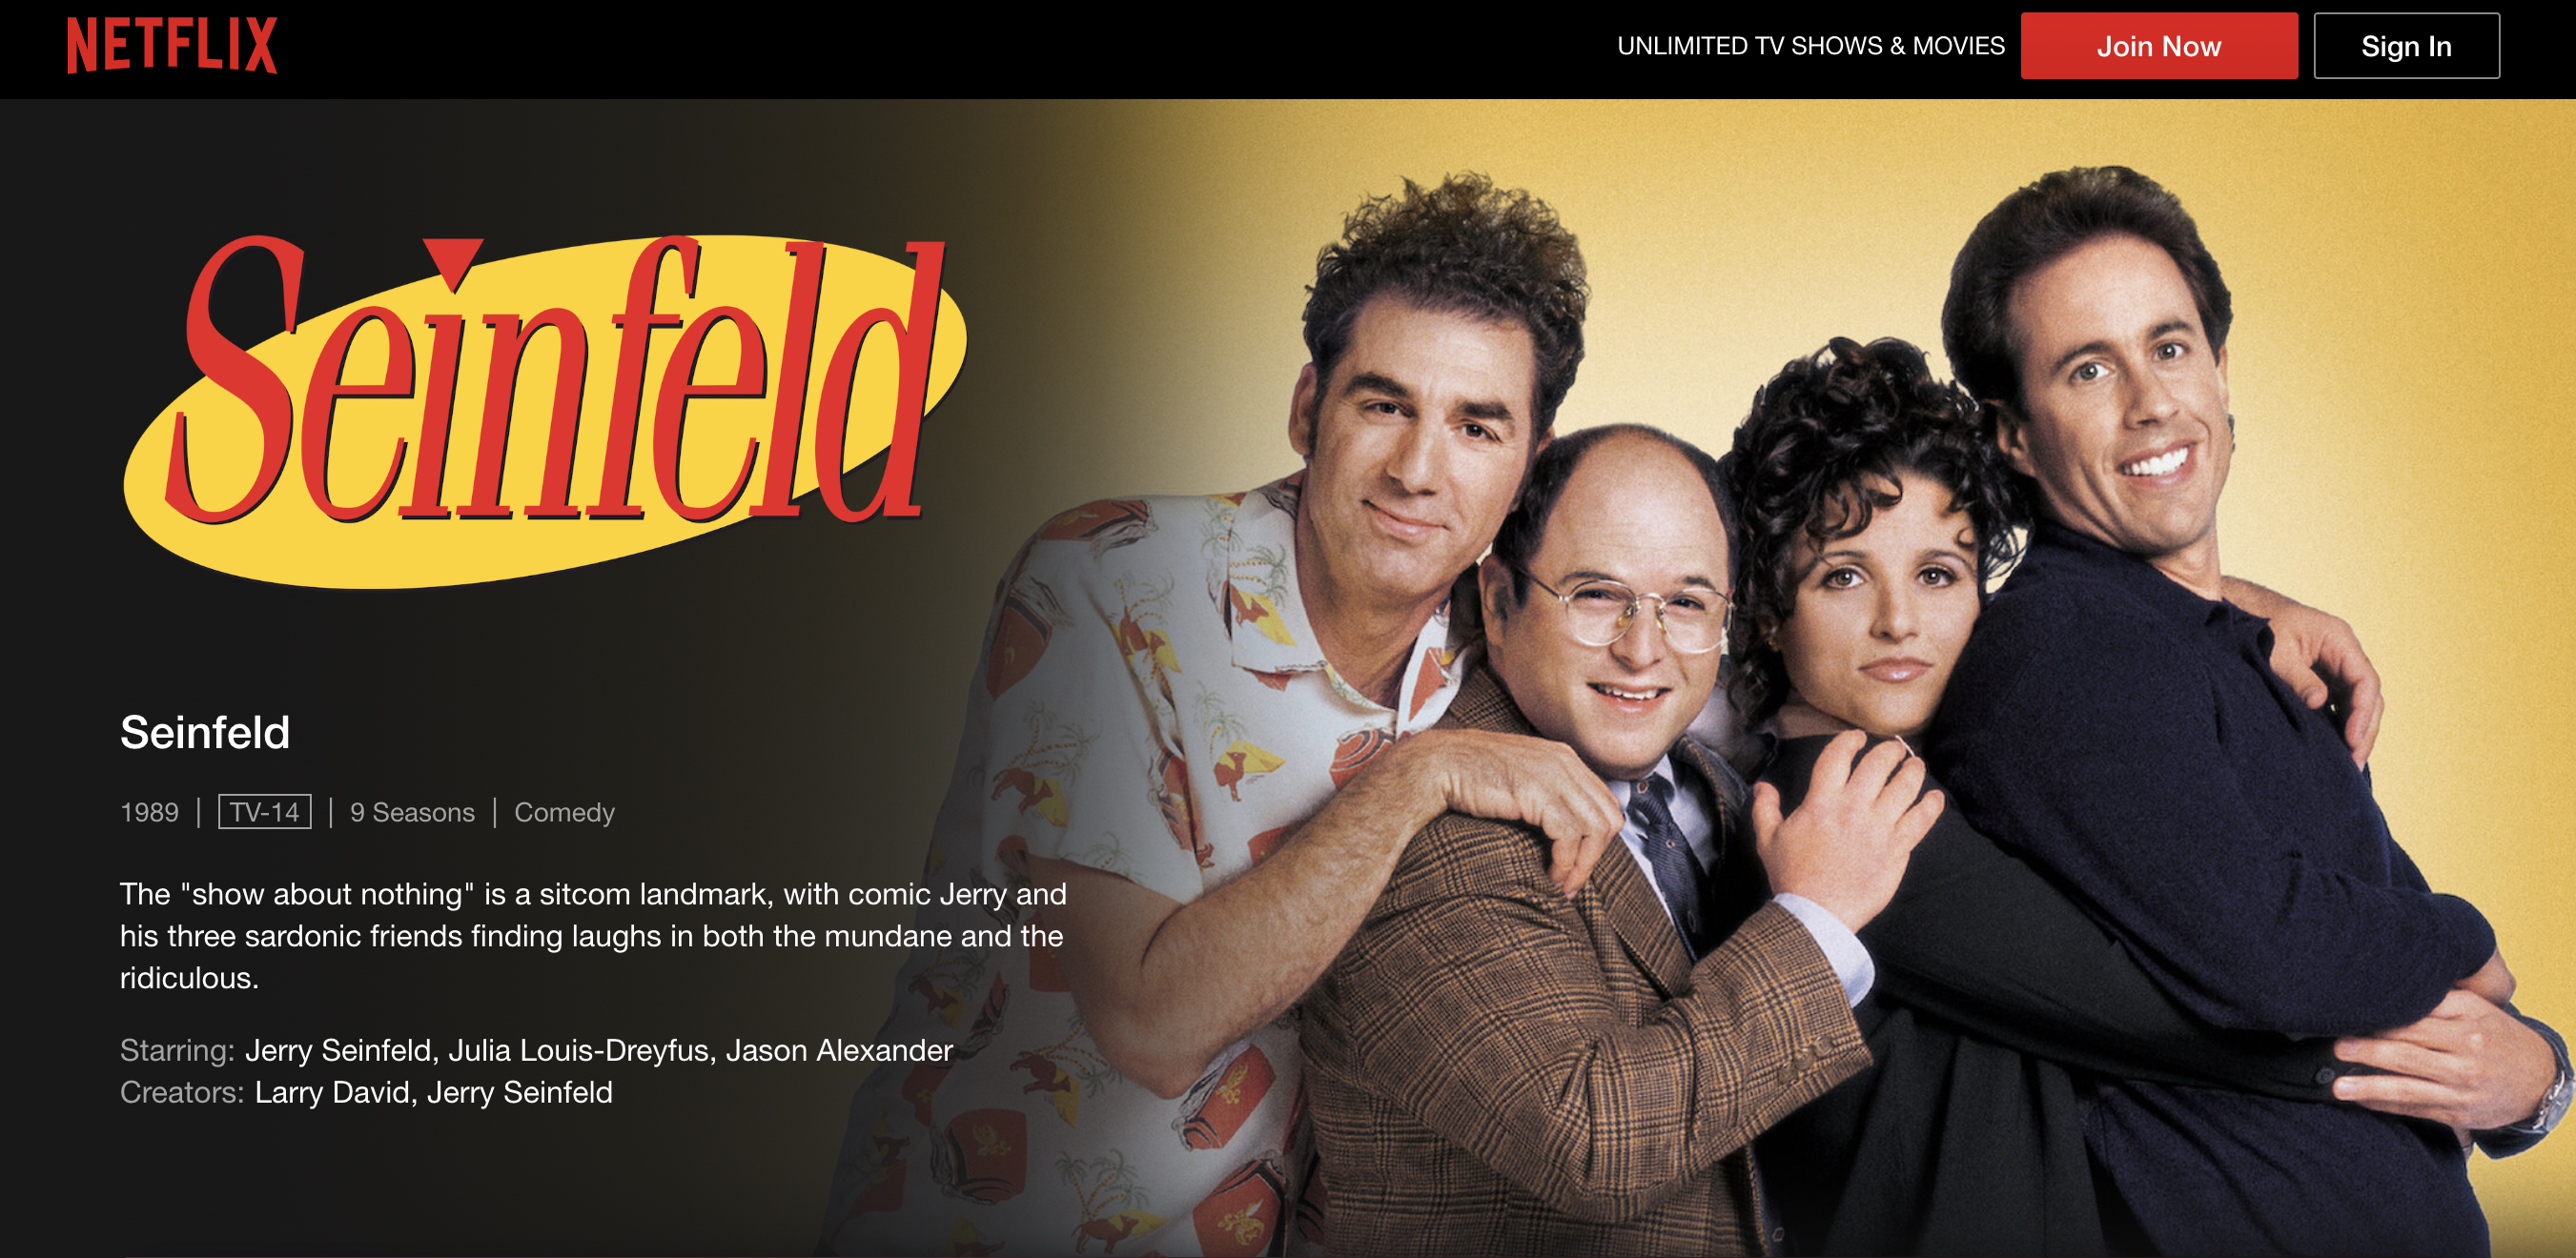
\includegraphics{img/seinfeld-netflix.jpg}}

Who doesn't love \textbf{Seinfeld}, the classic sitcom show
\textbf{about nothing} that was the benchmark for TV comedy in the
1990s? Now that all 9 seasons are streaming on
\href{https://www.netflix.com/title/70153373}{Netflix}, Gen Zers who are
too young to have seen the show when it was first aired can enjoy it in
all its glory. As anyone familiar with the show knows, the premise of
the show itself was that it was a show ``about nothing''---early in its
history there was even a very ``meta'' series of episodes in which Jerry
and George pitch their idea for a comedy ``about nothing'' to executives
at NBC--the very network that was actually airing those episodes!

Which is why it's strangely appropriate that the show is the
reference-point for one of the stranger forms of ``content'' to have
swum across my screen in recent years: a procedurally-generated,
never-ending animated version of the show that began streaming on the
Twitch gaming platform last year, titled---appropriately
enough---\href{https://www.twitch.tv/watchmeforever}{\textbf{Nothing,
Forever}}.

I mention this example for a number of reasons. First, because it's a
perfect example of the content category that Kate Eichhorn defines as
\textbf{entertainment content} in the first chapter of her recent book
on the subject. Back in the 1990s, \textbf{Seinfeld} was airing at the
exact same time that Bill Gates first published his famous essay,
``Content is King'' (referenced in Patrick Willem's YouTube video on the
same subject). Yet as prescient as that essay may now seem in
retrospect, the term ``content'' was still far from taking on the
specific meaning that it began to about a decade later, while nobody at
the time would have dreamed of describing \textbf{Seinfeld} as
\textbf{content}: it was simply \textbf{television}. The distance
between then and now is a measure of how far digital media and the
emergence of the World Wide Web (as it was still called when
\textbf{Seinfeld} was airing on NBC) have tranformed the nature of
entertainment over the intervening quarter century. For in contrast to
its 1990s TV source, \textbf{Nothing, Forever} is a quintessential
example of what we mean today by the term \textbf{content}: a media text
whose cultural value resides primarily---if not exclusively---in its
capacity to \textbf{circulate} widely across the social mediascape. In
that respect, \textbf{Nothing, Forever} can be seen as a counterpart to
the Instagram egg account that provides the starting-point for Kate
Eichhorn's discussion of content. And like its counterpart, the
Twitchstream show quickly began to propagate beyond the specific
platform on which it originated. In addition to the torrent of online
chatter it generated on tech news sites and social media platforms like
Reddit, it quickly spawned the by now all-too-familiar YouTube
spin-offs: a best-of compilation, a
\href{https://www.youtube.com/playlist?list=PLMWNMOWqRRvAiIIjXuxsxEpOXw3GV2b6G}{playlist
of archived episodes}, and numerous dystopian predictions by social
media commentators of how the show was a harbinger of the imminent tidal
wave of generative-AI content about to break over our heads.

\url{https://www.youtube.com/embed/yn0iVOtr6FE}

Other than the fact that it was animated rather than a live-action
sitcom, this is, of course, the most significant difference between
\textbf{Nothing, Forever} and its televisual source. Remediated on
Netflix, the original collection of TV episodes that comprise the
original \textbf{Seinfeld} series were transmuted into \textbf{content}:
just another batch of archival TV shows on the shelf of the vast library
of ``classic'' or ``vintage'' TV, not to mention all of the comedy
series since. This reductive ``flattening'' of content, in which one
show becomes functionally no different from any other is, as Patrick
Willems explains in his YouTube video, one of the most insidious aspects
of the concept of content in itself, and the basis for his critique of
it.

But of course, \textbf{Nothing, Forever} is not just content in the same
way that \textbf{Seinfeld} itself becomes content in the age of
streaming media: it's particular distinctive quality is that it's also
\textbf{generative} content, or more specifically that it's
\textbf{procedurally} generated sourced from the raw materials of the
original show itself. This generative automation of its content is both
\textbf{continuous} and---at least in principle---
\textbf{interminable}, in that content can be algorithmically generated
in this way \textbf{ad infinitum}: unlike its network-TV-era source,
unlike even its on-demand streaming remediation, \textbf{Nothing
Forever} was an early example of a new development in popular
entertainment in the age of AI: \textbf{infinite content}. Rather than
the gnarly animated visuals and stilted dialogue, it's this generative
dimension of the show that cultural critics seemed to find most
disturbing: that as the title made clear, \textbf{it could go on
forever}. What dire implications did this have for the
actually-existing, still human-based entertainment industry? Could it be
seen as a sign of the beginning of the end of that industry in itself?
Certainly there have been no shortage of media commentators to have
claimed that this is precisely the threat posed by AI-generated content
to the creative industries in general. My own view is that the backlash
against AI that has quickly taken hold in the entertainment industry
over the past year or two---as seen in the recent industrial action of
the writers' and actors' guilds--may prove to have over-stated the
doomsday scenarios that have been circulating. I'd be interested to hear
your thoughts on that issue!

Speculations about the future of the content industry aside, what is
clear in the present is that generative content of the type exemplified
by \textbf{Nothing, Forever} currently represents the leading edge of
creative experimentation with algorithmic technologies. But the tsunami
of AI-generated entertainment has already begun to break, most notably
on YouTube itself, which currently hosts a rapidly-growing corpus of
AI-generated movies using contemporary neural networks (aka
``large-language models'' or LLMs) like Runway, Sora, ComfyUI, and many
more. (This topic is also explored by Kate Eichhorn in the concluding
chapter of her book.)

Let me conclude with what may seem like a counter-intuitively positive
pointt about generative entertainment content. In the midst of the
current and ongoing furore about the onset of what might be called the
age of \textbf{procedural media} aspect has been overlooked: its social
role as a catalyst for generating new forms of \textbf{creative
community}. One interesting element of the Twitchstream version of
\textbf{Nothing, Forever} was that it was accompanied by a live-feed
chat of people talking about and responding to the show in real time.
Significantly, no such real-time chat was available on Netflix for
streaming re-runs of the original \textbf{Seinfeld} series.
\textbf{Nothing, Forever} also sparked intense discussion on Reddit in
the generative sub-group, as well as elsewhere across the social
mediascape.

In the end, old-school media studies questions about audience, and
whether anyone was actually watching \textbf{Nothing, Forever} the way
TV audiences back in the 1990s had gathered to watch \textbf{Seinfeld}
when it aired, are moot. The Twitch show simply belongs to a very
different media species, in which the primary purpose of
content--whether generative or otherwise---is catalytic, serving not
just to circulate but to generate social interaction and community. If
you look around online, you will see many examples of such content.
Contrary to what is often assumed, this content is highly effective in
generating further chains of content---memes are a good example.

So in conclusion, I would suggest that in addition to the categories of
content defined by Kate Eichhorn in the first chapter of her
book---Marketing Content, Entertainment Content, Educational Content,
User-Generated Content, etc.--we may add a further one:
\textbf{Meta-Content}. Meta-Content is content where the buzz or
discourse around a particular kind of content is at least as significant
as the source content that produced it. From that perspective the
``buzz'' around \textbf{Nothing, Forever} was as much a part of its
content as the actual show itself. In a way, when it comes to
Meta-Content the nature of the content ``itself'' is almost
arbitrary---it doesn't matter all that much what it is, as long as it
captures people's attention and spawns larger conversations---or better
still, controversies. If this hypothesis is correct, it's all the more
interesting---and ironic---that the show that may be remembered as one
of the inaugural examples of generative content is a show about
\textbf{nothing}. While there may be nothing--or at most hardly
anything--to watch, there is certainly plenty to talk about, and in the
age of Meta-Content, that is all that matters.

I'll leave you with one last example of another new form of
(Meta-)content that has also begun to emerge from the media laboratory
known as YouTube: satirical commentary on AI creativity itself. You may
enjoy this amusing reflection on the possible future into which we may
be heading, and the strange new kinds of creative practices that may
emerge from it.

\url{https://www.youtube.com/embed/N_Nvr4ztBXs}

\begin{center}\rule{0.5\linewidth}{0.5pt}\end{center}




\end{document}
